\documentclass{beamer}

\usepackage{txfonts}
\usepackage{hyperref}
\usepackage{fancybox}
\usepackage{xfrac}
\usepackage{cancel,slashbox}

\newcommand{\heart}{\ensuremath\heartsuit}

\usepackage{mathtools,amssymb}
\newcommand{\myarrow}{\scalebox{2}[2]{$\mathclap{\curvearrowleft}\mkern2.2mu
                                                 \mathclap{\curvearrowright}$}}

\DeclareMathOperator{\Bin}{\mathrm{Bin}}
\DeclareMathOperator{\Max}{\mathrm{Max}}

\hypersetup{colorlinks=false,linkbordercolor=red,linkcolor=green,pdfborderstyle={/S/U/W 1}}

\addtobeamertemplate{navigation symbols}{}{ \hspace{1em}    \usebeamerfont{footline}%
    \insertframenumber / \inserttotalframenumber}

\geometry{papersize={15cm,15cm}}
\usepackage{lipsum}

\makeatletter
\newenvironment<>{contdproof}[1][\proofname]{%
    \par
    \def\insertproofname{#1\@addpunct{.}}%
    \usebeamertemplate{proof begin}#2}
  {\usebeamertemplate{proof end}}
\makeatother


\setbeamertemplate{theorems}[numbered]

\newtheorem{remark}{Remark}



\newtheorem*{nonumdefinition}{Definition}
\newtheorem*{nonumproblem}{Problem}
\newtheorem*{nonumcorollary}{Corollary}
\newtheorem*{nonumlemma}{Lemma}
\newtheorem*{nonumproof}{Proof}
\newtheorem*{nonumtheorem}{Theorem}
\newtheorem*{nonumremark}{Remark}
\newtheorem*{answer}{Answer}
\newtheorem*{nonumremarks}{Remarks}
\newtheorem*{nonumexamples}{Examples}
\newtheorem*{nonumsolution}{Solution}
\newtheorem*{nonumexample}{Example}
\newtheorem*{nonumproposition}{Proposition}
\newtheorem{proposition}[theorem]{Proposition}

\usepackage{tikz}
\newcommand*\mycirc[1]{%
  \tikz[baseline=(C.base)]\node[draw,circle,inner sep=.7pt](C) {#1};\:
}

\newcommand\myheading[1]{%
  \par\bigskip
  {\color{blue}{\large #1}}\par\smallskip}

%\usetheme{Warsaw}
%\usetheme{Berkeley} %sample 1

\usetheme{Berlin} % sample 2
%\usetheme{AnnArbor} % sample 3

\let\otp\titlepage
\renewcommand{\titlepage}{\otp\addtocounter{framenumber}{-1}}

\title{Lecture 15 : Pairs of Discrete Random Variables}
\author{}
\date{}

\begin{document}
\begin{frame}[plain]
\titlepage
\end{frame}

\begin{frame}
Today we start Chapter 5. The transition we are making is like going from one variable calculus to vector calculus. We should really think of vectors $(X,Y)$ of random variables.

So suppose $X$ and $Y$ are discrete random variables defined on the same sample space $S$.

\begin{nonumdefinition}
The \underline{joint} probability mass function, joint $pmf$, $P_{X,Y}(x,y)$, is defined by

\smallskip
\centerline{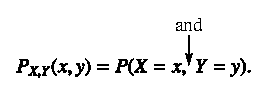
\includegraphics{figure/fig1.eps}}
\end{nonumdefinition}
\end{frame}

\begin{frame}
\begin{nonumexample}
A fair coin is tossed three times.

Let

\qquad $X=\sharp$ of head on first toss

\qquad $Y=\text{~total~}\sharp$ of heads

As usual
$$
S=\left\{
\begin{array}{l}
HHH, \ HHT, \ HTH, \ HTT\\
THH, \ THT, \ TTH, \ TTT
\end{array}
\right\}
$$
We want to compute
\begin{align*}
P_{X,Y}(x,y) &= P(X=x, Y=y)\\
            &= P((X=x)\cap (Y=y))\\
            &= P(X=x)P(Y=y|X=x)
\end{align*}
\end{nonumexample}
\end{frame}

\begin{frame}
We will record the results in a matrix which we will now compute

\smallskip
\centerline{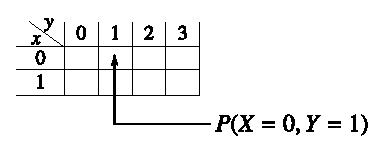
\includegraphics{figure/fig2.eps}}
\smallskip

\myheading{First column $(y=0)$}

Let's compute (upper left, $x=0$)

\smallskip
\centerline{\includegraphics{figure/fig3.eps}}
\smallskip

Now lower left $(X=1)$

$P_{X,Y}(1,0)=P(X=1,Y=0)=0$

\myheading{Move to the $2^{\text{nd}}$ column $(y=1)$}

$P_{X,Y}(0,1)=P(X=0,Y=1)$\quad (top entry $X=0$)
\end{frame}

\begin{frame}
This is harder
\begin{align*}
P(X=0,Y=1) &= P(T\text{~on first and exactly 1 head total})\\
           &= P(THT)+P(TTH)=\dfrac{2}{8}
\end{align*}
The bottom entry of the second column is
$$
P(X=1,Y=1)=P(HTT)=\dfrac{1}{8}
$$

\myheading{Third column $(y=2)$}
\begin{align*}
P(X=0,Y=2) &= P(THH)=\dfrac{1}{8}\\
P(X=1,Y=2) &= P(HTH)+P(HHT)\\
           &=\dfrac{2}{8}
\end{align*}

\myheading{Fourth column $(y=3)$}
\begin{align*}
P(X=0,Y=3) &=0\\
P(X=1,Y=3) &= P(HHH)=\dfrac{1}{8}
\end{align*}
\end{frame}

\begin{frame}
\myheading{The table for the joint $pmf$ $P_{X,Y}(x,y)$}

\begin{equation*}
{\renewcommand{\arraystretch}{1.2}
\begin{array}{c|c|c|c|c|}
\text{\backslashbox{$X$}{$Y$}} & 0 & 1 & 2 & 3\\
\hline
0 & \frac{1}{8} & \frac{2}{8} & \frac{1}{8} & 0\\
\hline
1 & 0 & \frac{1}{8} & \frac{2}{8} & \frac{1}{8}\\
\hline
\end{array}}\tag{*}\label{eq-*}
\end{equation*}
Check that the total probability is 1. 

The joint $pmf$ has a huge amount of information in it. In particular it contains the $pmf$ $P_{X}(x)$ of $X$ and $P_{Y}(y)$ of $Y$.

So how do we recover $P(Y=1)$ from the table above. The event $(Y=1)$ is the union of the two events $(X=0,Y=1)$ and $(X=1,Y=1)$. These two are mutually exclusive.
\end{frame}

\begin{frame}
So
\begin{align*}
P(Y=1) &= P(X=0,Y=1)+P(X=1,Y=1)\\
       &= \frac{2}{8}+\frac{1}{8}=\frac{3}{8}
\end{align*}
= the sum of the entries in the second \underline{column} (i.e. the column corresponding to $y=1$)

\myheading{How about $P(X=1)$?}

We have an equality of events
\begin{align*}
(X=1) &= (X=1,Y=0)\cup (X=1,Y=1)\cup (X=1,Y=2)\cup (X=1,Y=3)\\
      &= 0+\frac{1}{8}+\frac{2}{8}+\frac{1}{8}=\frac{1}{2}\\
      &= \text{the sum of the entries in the second \underline{row} (corresponding to $X=1$)}
\end{align*}
\end{frame}

\begin{frame}
So we see we recover $P_{Y}(y)$ by taking \underline{column sums} and $P_{X}(x)$ by taking \underline{row sums}.

\myheading{Marginal Distributions}

We can express the above nicely by expanding the table \eqref{eq-*} ``adding margins''.

\myheading{Table \eqref{eq-*} with margins added}
\begin{equation*}
{\renewcommand{\arraystretch}{1.2}
\begin{array}{c|c|c|c|c|}
\text{\backslashbox{$x$}{$y$}} & 0 & 1 & 2 & 3\\
\hline
0 & \frac{1}{8} & \frac{2}{8} & \frac{1}{8} & 0\\
\hline
1 & 0 & \frac{1}{8} & \frac{2}{8} & \frac{1}{8}\\
\hline
  & & & &\\
\end{array}}\tag{**}\label{eq-**}
\end{equation*}
\end{frame}

\begin{frame}
\myheading{The \S64,000 question}

How do you fill in the margins?

There is only one reasonable way to do this --- put the row sums in the right margin and the column sums in the bottom margin.

\myheading{Table \eqref{eq-**} with the margins filled in}
\begin{equation*}
{\renewcommand{\arraystretch}{1.2}
\begin{array}{c|c|c|c|c|c}
\text{\backslashbox{$x$}{$y$}} & 0 & 1 & 2 & 3 & \\
\hline
0 & \frac{1}{8} & \frac{2}{8} & \frac{1}{8} & 0 & \frac{1}{2}\\
\hline
1 & 0 & \frac{1}{8} & \frac{2}{8} & \frac{1}{8} & \frac{1}{2}\\
\hline
  & \frac{1}{8} & \frac{3}{8} & \frac{3}{8} & \frac{1}{8} & \\
\end{array}}\tag{**{*}}\label{eq-***}
\end{equation*}
\end{frame}

\begin{frame}
The right margin tells us the $pmf$ of $X$ and the bottom margin tells us the $pmf$ of $Y$.
\begin{center}
\renewcommand{\arraystretch}{1.2}
\begin{tabular}{|c|c|c|}
$X$ & & \\
\cline{1-1} 
\cline{3-3}
$0$ & \ldots & $\frac{1}{2}$\\
\cline{1-1} 
\cline{3-3}
$1$ &        & $\frac{1}{2}$\\
\cline{1-1} 
\cline{3-3}
\end{tabular}
\end{center}

\begin{center}
\renewcommand{\arraystretch}{1.2}
\begin{tabular}{c|c|c|c|c|}
$y$ & 0 & 1 & 2 & 3\\
\hline
\multicolumn{5}{c}{$\vdots$}\\
\hline
 & $\frac{1}{8}$ & $\frac{3}{8}$ & $\frac{3}{8}$ & $\frac{1}{8}$
\end{tabular}
\end{center}
So we have
\begin{center}
\begin{minipage}[c]{4cm}
\begin{tabular}{c|c|c|}
$x$ & 0 & 1\\
\hline
$P(X=x)$ & $\dfrac{1}{2}$ & $\dfrac{1}{2}$\\
\hline
\end{tabular}
\end{minipage}
\begin{minipage}[c]{1cm}
and
\end{minipage}
\begin{minipage}[c]{4cm}
\begin{tabular}{c|c|c|c|c|}
$y$ & 0 & 1 & 2 & 3\\
\hline
$P(Y=y)$ & $\dfrac{1}{8}$ & $\dfrac{3}{8}$ & $\dfrac{3}{8}$ & $\dfrac{1}{8}$\\
\hline
\end{tabular}
\end{minipage}
\end{center}

\centerline{$X\sim \Bin\left(1,\dfrac{1}{2}\right)$\hspace{3cm} $Y\sim \Bin\left(3,\dfrac{1}{2}\right)$}
\end{frame}

\begin{frame}
For this reason, given the pair $(X,Y)$ the $pmf$'s $P_{X}(x)$ and $P_{Y}(y)$ are called the marginal distributions.

To state all this correctly we have
\begin{nonumproposition}
\begin{itemize}
\item[(i)] $P_{X}(x)=\sum\limits_{\text{all~ }y}P_{X,Y}(X,y)\binom{\text{row}}{\text{sum}}$

\item[(ii)] $P_{Y}(y)=\sum\limits_{\text{all~ }x}P_{X,y}(x,y)\binom{\text{column}}{\text{sum}}$
\end{itemize}
So you ``sum away'' one variable leaving a function of the \underline{remaining variable}.
\end{nonumproposition}
\end{frame}

\begin{frame}
\myheading{Combining Discrete Random Variables}

Suppose $X$ and $Y$ are discrete random variables defined on the same sample space. Let $h(x,y)$ be a real-valued function of two variables. We want to define a new \underline{random variable} $W=h(X,Y)$.

\myheading{Examples}

We will start with the pair $(X,Y)$ from our basic example.

\underline{The key point is that a function of a pair of random variables}

\underline{is again a random variable.} 
\end{frame}

\begin{frame}
We will need only the joint $pmf$
\begin{equation*}
\renewcommand{\arraystretch}{1.2}
\begin{array}{c|c|c|c|c|}
\text{\backslashbox{$x$}{$y$}} & 0 & 1 & 2 & 3\\
\hline
0 & \frac{1}{8} & \frac{2}{8} & \frac{1}{8} & 0\\
\hline
1 & 0 & \frac{1}{8} & \frac{2}{8} & \frac{1}{8}\\
\hline
\end{array}\tag{*}\label{addeq-*}
\end{equation*}
\begin{itemize}
\item[(i)] $h(x,y)=x+y$\quad so\quad $W=X+Y$
\end{itemize}

We see that the possible values of the sum are $0,1,2,3,4$ (since they are the sums of the possible values of $X$ and $Y$).

We need to compute their probabilities. How do you compute
$$
P(W=0)=P(X+Y=0)?
$$

\begin{answer}
Find all the pairs $x$ and $y$ that add up to zero, take the probability of each such pair and add the resulting probabilities.
\end{answer}
\end{frame}

\begin{frame}
\begin{answer}[Cont.]
Bit $X+Y=0\Leftrightarrow X=0$ and $Y=0$ so there is only one such pair $(0,0)$ and (from the joint proof \eqref{addeq-*})
$$
P(X=0,Y=0)=\frac{1}{8}
$$
Hence
$$
P(W=0)=P(X=0,Y=0)=\frac{1}{8}
$$
\begin{align*}
P(W=1) &= P(X+Y=1)\\[3pt]
       &= P(X=0,Y=1)+P(X=1,Y=0)\\[3pt]
       &= \frac{2}{8}+0=\frac{2}{8}
\end{align*}
\begin{align*}
P(W=Z) &= P(X=0,Y=Z)+P(X=1,Y=1)\\[3pt]
       &= \frac{2}{8}
\end{align*}
\end{answer}
\end{frame}

\begin{frame}
\begin{answer}[Cont.]
Similarly
$$
P(W=3)=\frac{2}{8}\quad\text{and}\quad P(W=4)=\frac{1}{8}
$$
So we get for $W=X+Y$
\begin{equation*}
\renewcommand{\arraystretch}{1.2}
\begin{array}{c|c|c|c|c|c|}
W & 0 & 1 & 2 & 3 & 4\\
\hline
P(W=w) & \frac{1}{8} & \frac{2}{8} & \frac{2}{8} & \frac{2}{8} & \frac{1}{8}\\
\hline
\end{array}\tag{b}\label{eq-b}
\end{equation*}\label{page14}
(check that the total probability is $1$)
\end{answer}

\begin{nonumremark}
Technically the rule given in the ``Answer'' above is the \underline{definition} of $W=X+Y$ as a random variable but as usual the definition is forced on us.
\end{nonumremark}

\begin{itemize}
\item[(ii)] $h(X,y)=xy$\quad so\quad $W=XY$
\end{itemize}

The possible values of $W$ (the products of values of $X$ with those of $Y$) are $0,1,2,3$.
\end{frame}

\begin{frame}
We now compute their probabilities.

\myheading{P(W=0)}

We can get $0$ as a product $xy$ if either $x=0$ or $y=0$ so we have
\begin{align*}
P(W=0) &= P(XY=0)\\
       &= P(X=0,Y=0)+P(X=0,Y=1)+P(X=0,Y=2)\\
       &\quad +P(X=0,Y=3)+P(X=1,Y=0)\\
       &= \frac{1}{8}+\frac{2}{8}+\frac{1}{8}+0+0=\frac{1}{2}
\end{align*}

\myheading{P(W=1)}
$$
P(W=1)=P(X=1,Y=1)=\frac{1}{8}
$$
\end{frame}

\begin{frame}
\myheading{$P(W=2)$}
$$
P(W=2)=P(X=1,Y=2)=\frac{2}{8}
$$

\myheading{$P(W=3)$}
$$
P(W=3)=P(X=1,Y=3)=\frac{1}{8}
$$
\begin{center}
\renewcommand{\arraystretch}{1.2}
\begin{tabular}{c|c|c|c|c|}
\hline
$W$ & 0 & 1 & 2 & 3\\
\hline
$P(W=w)$ & $\frac{1}{2}$ & $\frac{1}{8}$ & $\frac{2}{8}$ & $\frac{1}{8}$\\
\hline
\end{tabular}
\end{center}

\begin{itemize}
\item[(iii)] $h(x,y)=\max (x,y)=\text{~the bigger of $x$ and $y$}$

so\quad $W=\max (X,Y)$
\end{itemize}

\begin{nonumremark}
The max function doesn't turn up in vector calculus but it turns up a lot in statistics in advanced mathematics and real life.
\end{nonumremark}
\end{frame}

\begin{frame}
The possible values of $\max (c,y)$ are $0,1,2,3$.

\myheading{$P(W=0)$}
\begin{align*}
P(W=0) &= P(\Max (X,Y)=0)\\
       &= P(X=0,Y=0)=\frac{1}{8}
\end{align*}

\myheading{$P(W=1)$}
\begin{align*}
P(W=1) &= P(\Max(X,Y)=1)\\
       &= P(X=0,Y=1)+P(X=1,Y=0)\\
       &\quad P(X=1,Y=1)=\frac{3}{8}
\end{align*}

\myheading{$P(W=2)$}
\begin{align*}
P(W=1) &= P(X=0,Y=2)+P(X=1,Y=2)\\
       &= \frac{3}{8}
\end{align*}
\end{frame}

\begin{frame}
\begin{align*}
P(W=3) &= P(X=0,Y=3)+P(X=1,Y=3)\\
       &= \frac{1}{8}
\end{align*}
\begin{center}
\begin{tabular}{c|c|c|c|c|}
$W$ & 0 & 1 & 2 & 3\\
\hline
$P(W=w)$ & $\frac{1}{8}$ & $\frac{3}{8}$ & $\frac{3}{8}$ & $\frac{1}{8}$\\
\hline
\end{tabular}
\end{center}
(check that the total probability is $1$)
\end{frame}

\begin{frame}
\myheading{The Expected Value of a Combination of Two Discrete Random Variables}

If $W=h(X,Y)$ there are two ways to compute $E(W)$.

\begin{nonumproposition}
\begin{equation*}
E(W) = \sum\limits_{\substack{\text{all~ }(x,y)\\ \text{possible}\\ \text{values of}\\ (X,Y)}} h(x,y)P_{X,Y}(x,y)\tag{$\sharp$}\label{eq-sharp}
\end{equation*}
We will illustrate the proposition by computing $E(W)$ for the $W=X+Y$ of pages $12$, $13$, $14$. 
\end{nonumproposition}

In \underline{two ways?}
\end{frame}

\begin{frame}
\myheading{First way (without using the proposition)}

$W$ is a random variable with proof given by \eqref{eq-b} on page 14.

(so we use \eqref{eq-b})
\begin{align*}
E(W) &= (0)\left(\dfrac{1}{8}\right)+(1)\left(\dfrac{2}{8}\right)+(2)\left(\frac{2}{8}\right)\\
     &\quad +(3)\left(\dfrac{2}{8}\right)+(4)\left(\dfrac{1}{8}\right)\\
     &=\frac{2+4+6+4}{8}=\frac{16}{8}=2
\end{align*}

\myheading{Second way (using the proposition)}

Now we use \eqref{addeq-*} from page 12
$$
E(W)=E(X+Y) = \underbrace{\sum\limits_{\text{all~ }x,y}(x+y)P_{X,Y}(x,y)}_{\substack{\text{sum over the 8 entries}\\ \text{of  \eqref{addeq-*}}}}
$$
\end{frame}

\begin{frame}
\begin{align*}
&= (0+0)\left(\dfrac{1}{8}\right)+(0+1)\left(\dfrac{2}{8}\right)+(0+2)\left(\dfrac{1}{8}\right)+(0+3)(???)\\
&\quad (1+0)(0)+(1+1)\left(\dfrac{1}{8}\right)+(1+2)\left(\dfrac{2}{8}\right)+(1+3)\left(\dfrac{1}{8}\right)\\
&= \frac{2+2}{8}+\frac{2+6+4}{8}\\
&= \frac{4+12}{8}=2
\end{align*}
The first way is easier but we need to compute the proof of $W=X+Y$ first. That was hard work, pages 12-14.
\end{frame}

\end{document}


